\section{Visualizers}
\subsection{LU Visualizer}
\subsubsection{Example 1: No arguments}{
\begin{lstlisting}[language=Python]
from BNumMet.Visualizers.LUVisualizer import LUVisualizer
luVisualizer = LUVisualizer()
display(luVisualizer.run())
\end{lstlisting}

\begin{enumerate}
  \item Initial State:\\  
    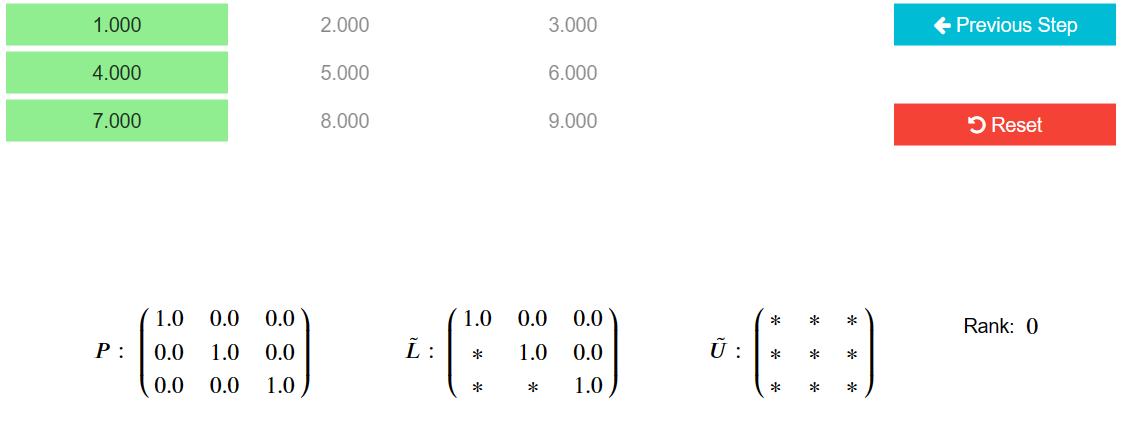
\includegraphics[scale=0.45]{Include/Images/Thesis/Documentation/Visualizers/LUVisualizer/Example 1/Example 1 - 00 - Initial State.png}
  \item Click on first column, second row:\\
    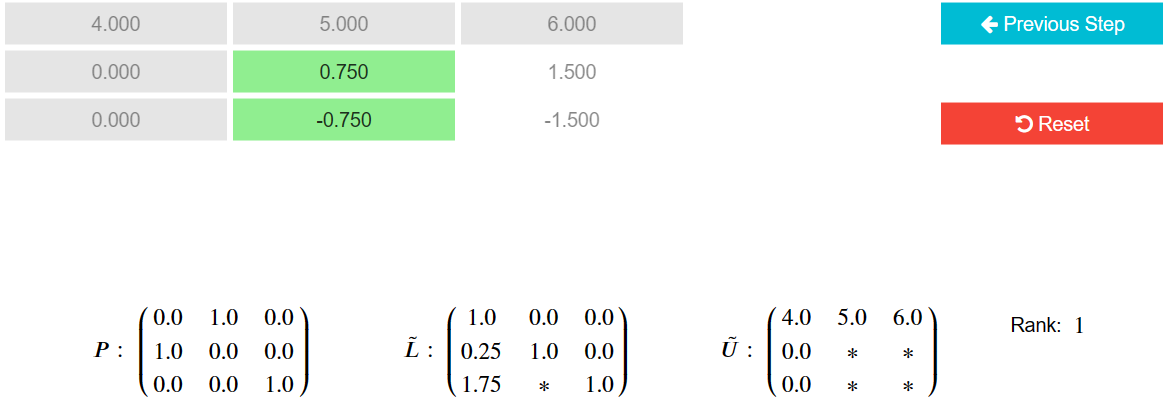
\includegraphics[scale=0.45]{Include/Images/Thesis/Documentation/Visualizers/LUVisualizer/Example 1/Example 1 - 01 - Click on 2 row.png}
  \item Click on second column, third row:\\
    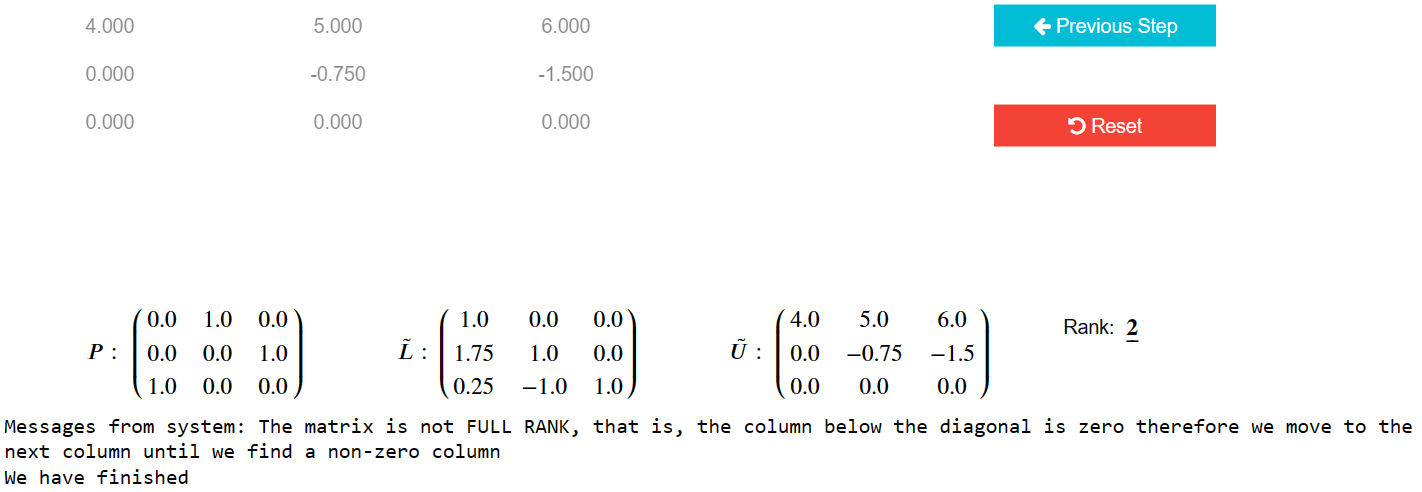
\includegraphics[scale=0.4]{Include/Images/Thesis/Documentation/Visualizers/LUVisualizer/Example 1/Example 1 - 02 - Click on 3 row.png}
  \item Click Previous Step:\\
    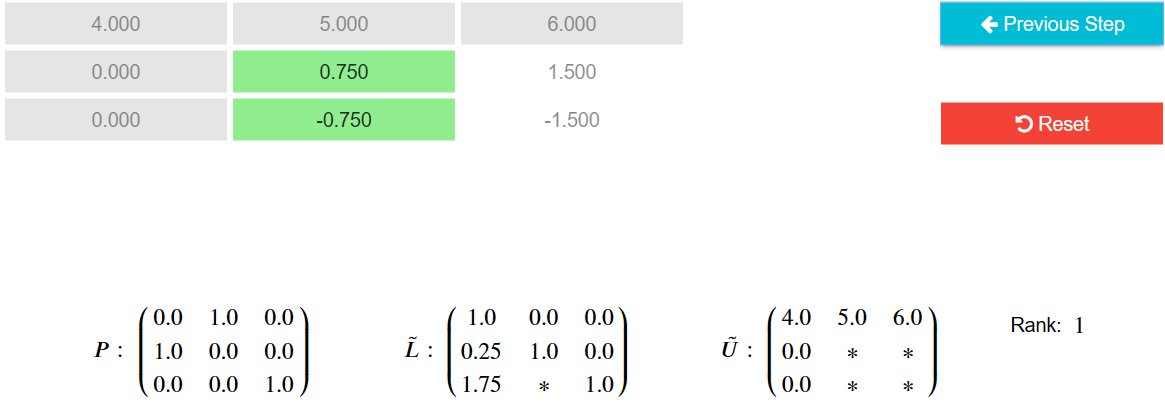
\includegraphics[scale=0.45]{Include/Images/Thesis/Documentation/Visualizers/LUVisualizer/Example 1/Example 1 - 03 - Click Previous Step.png}
  \item Click on second column, second row:\\
    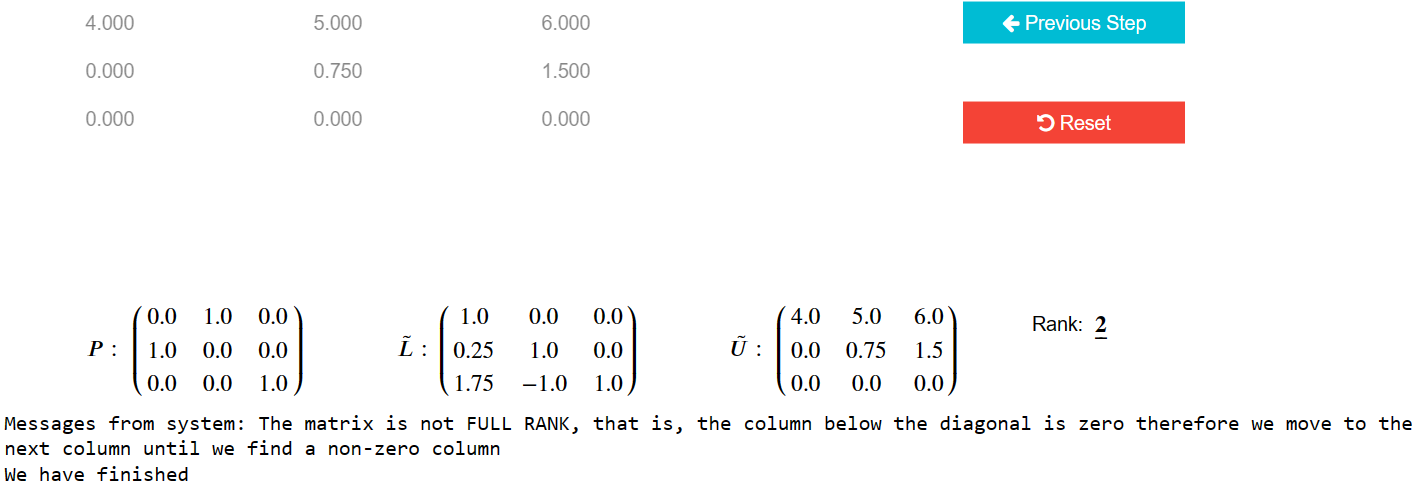
\includegraphics[scale=0.4]{Include/Images/Thesis/Documentation/Visualizers/LUVisualizer/Example 1/Example 1 - 04. - Click on 2 row.png}
  \item Click on Reset\\
      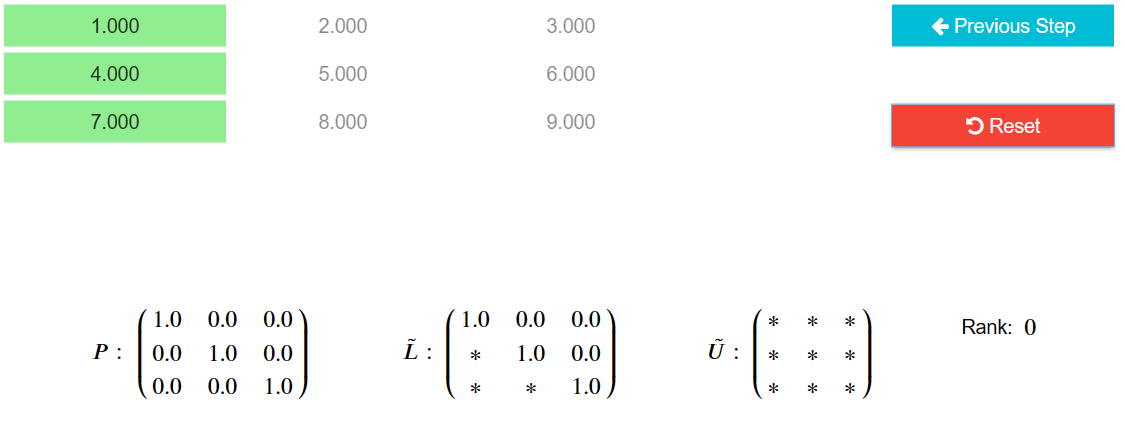
\includegraphics[scale=0.45]{Include/Images/Thesis/Documentation/Visualizers/LUVisualizer/Example 1/Example 1 - 05 - Click on Reset.png}
\end{enumerate}
}
\subsubsection{Example 2: Arguments and Rank Revealing}{
\begin{lstlisting}[language=Python]
from BNumMet.Visualizers.LUVisualizer import LUVisualizer
A = np.array([[1,2,3,7], [1,2,3,7], [1,2,3,7],[1,2,4,7]], dtype=float)
luVisualizer = LUVisualizer(A)
display(luVisualizer.run())
\end{lstlisting}

\begin{enumerate}
\item Initial State: \\
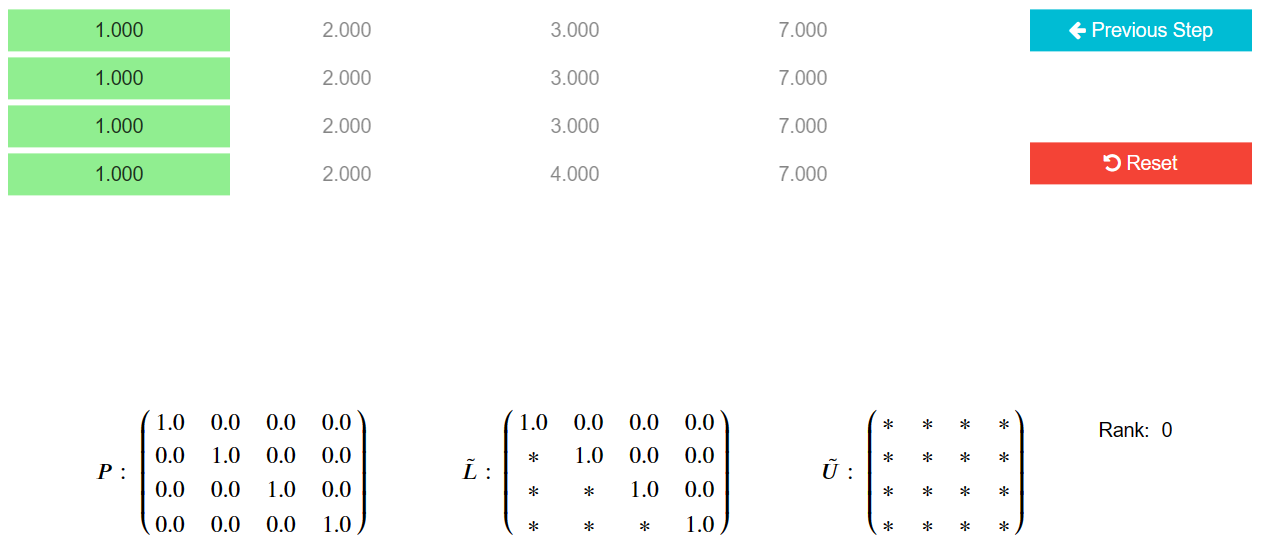
\includegraphics[scale=0.45]{Include/Images/Thesis/Documentation/Visualizers/LUVisualizer/Example 2/Example 2 - 00 - Initial State.png}

\item Click on the first column, second row: \\
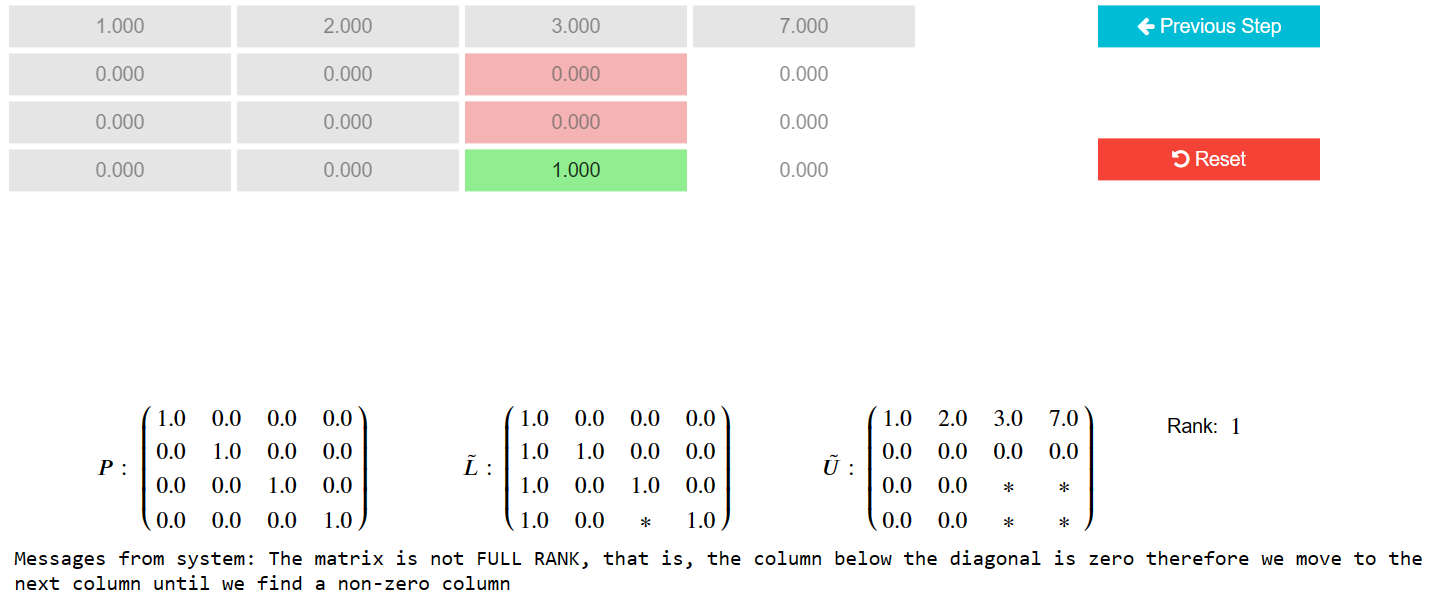
\includegraphics[scale=0.4]{Include/Images/Thesis/Documentation/Visualizers/LUVisualizer/Example 2/Example 2 - 01 - Click first column, second row.png}

\item Click on the third column, fourth row: \\
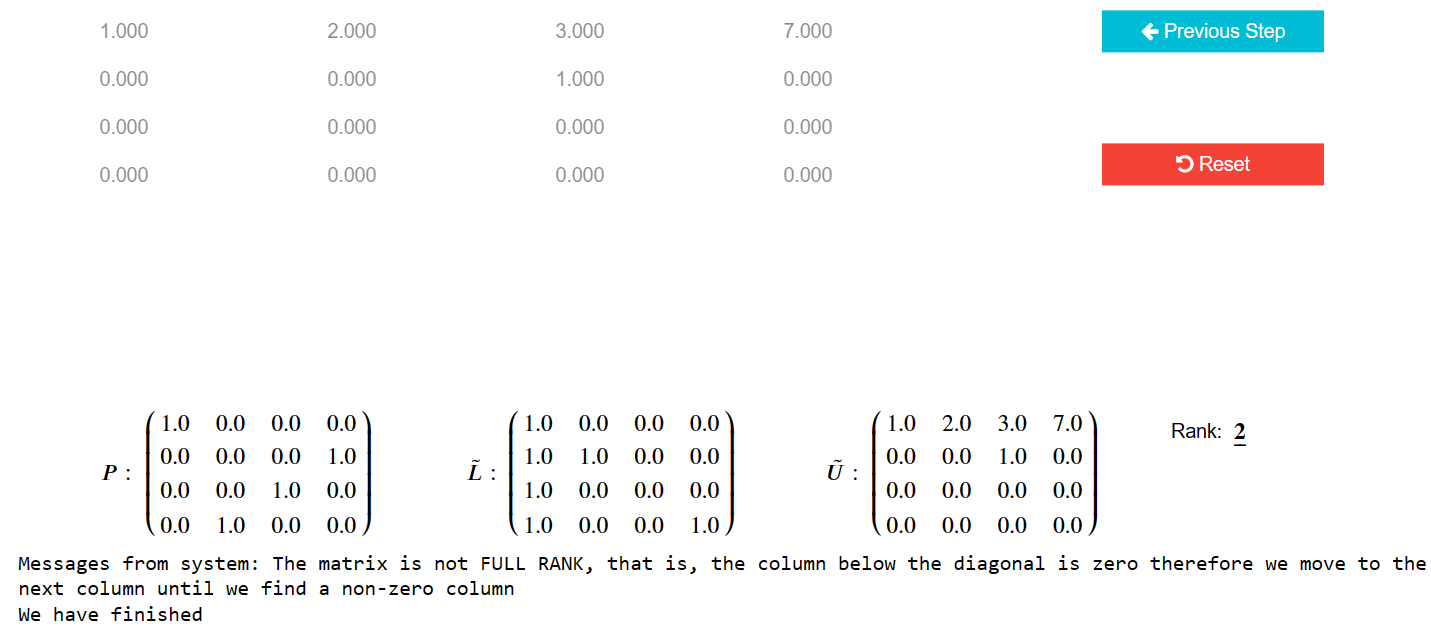
\includegraphics[scale=0.45]{Include/Images/Thesis/Documentation/Visualizers/LUVisualizer/Example 2/Example 2 - 02 - Click thirdcolumn, fourth row.png}
\end{enumerate}
}


\subsection{Interpolation Visualizer}
\subsubsection{Example 1}
\begin{lstlisting}[language=Python]
from BNumMet.Visualizers.InterpolationVisualizer import InterpolVisualizer
interpolVisualizer = InterpolVisualizer()
display(interpolVisualizer.run())
\end{lstlisting}
\begin{enumerate}
\item Initial State: \\
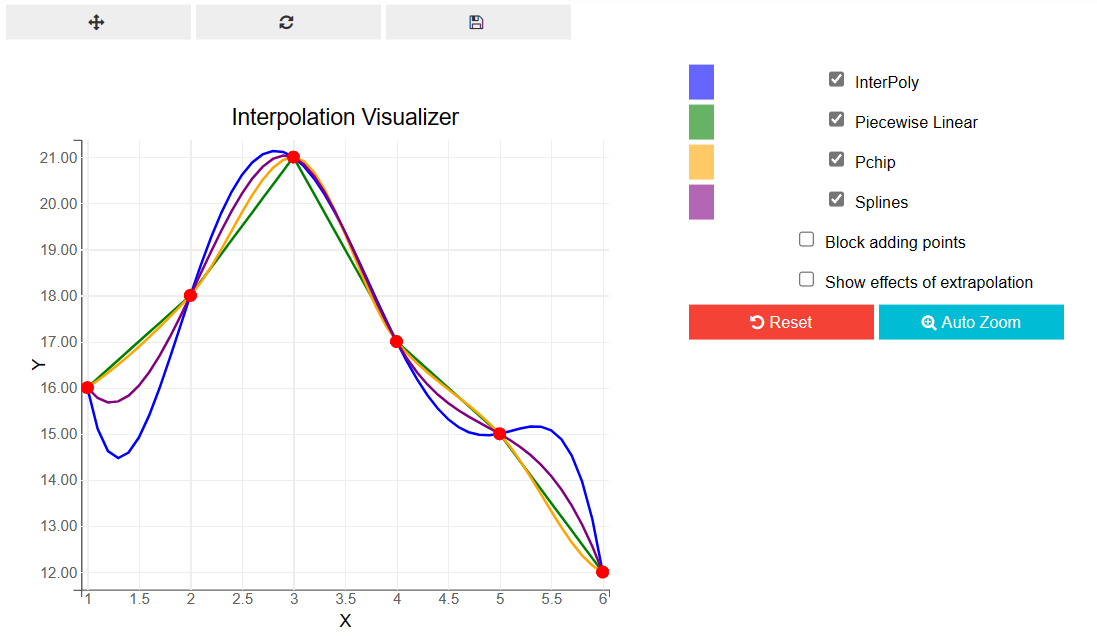
\includegraphics[scale=0.5]{Include/Images/Thesis/Documentation/Visualizers/Interpolation/Example 1/Example 1 - 00 - Initial State.png}

\item Checked Box Extrapolation and AutoZoom: \\
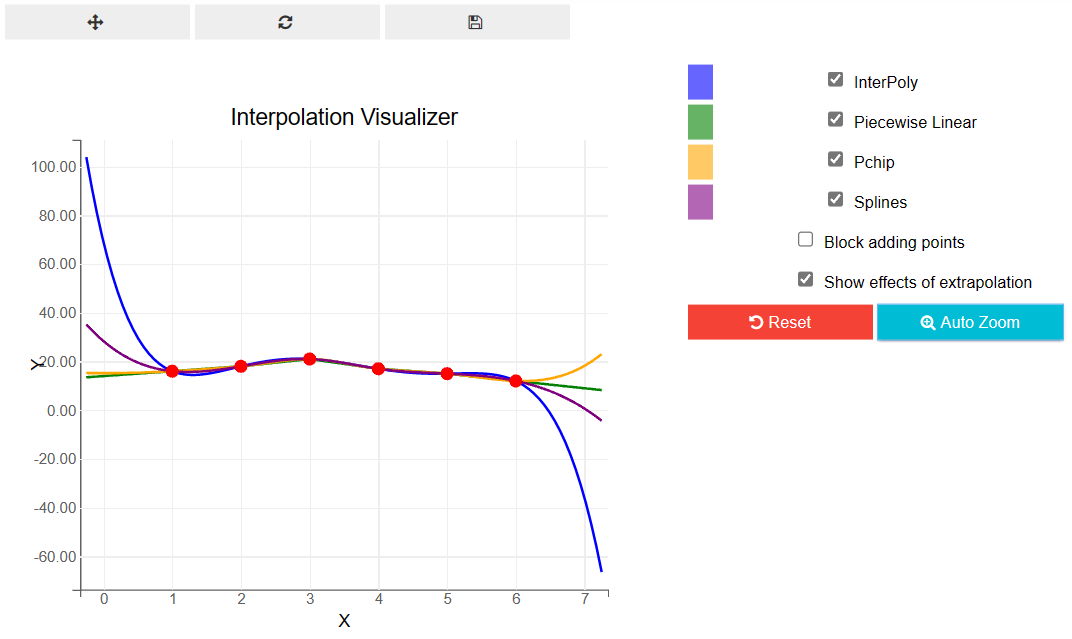
\includegraphics[scale=0.5]{Include/Images/Thesis/Documentation/Visualizers/Interpolation/Example 1/Example 1 - 01 - Checked Box Extrapolation and AutoZoom.png}

\item Reset Button: \\
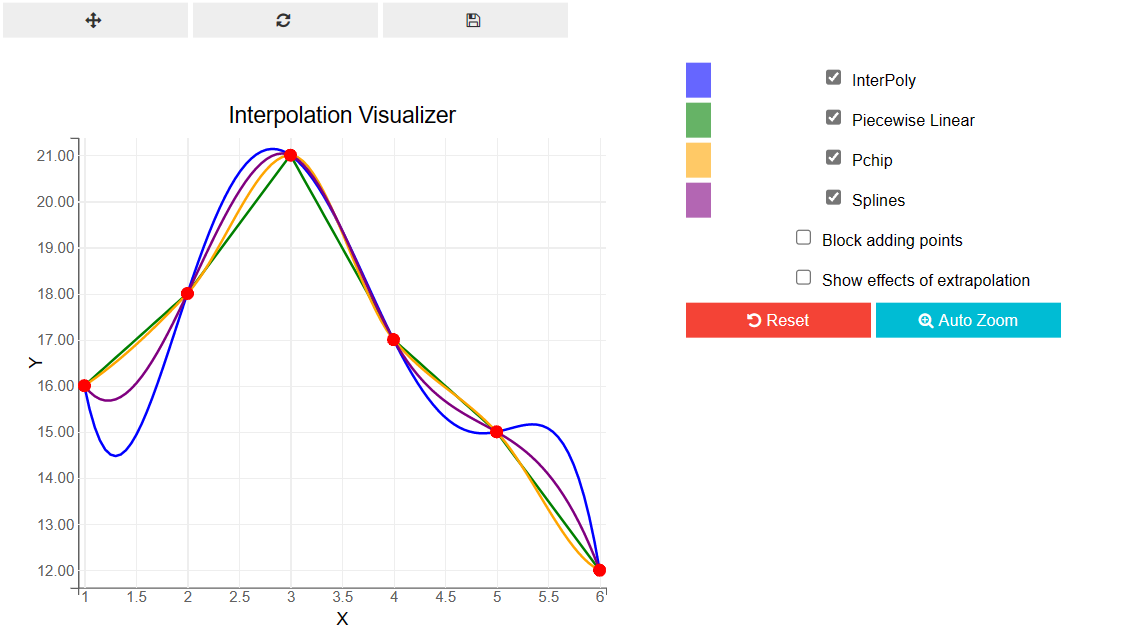
\includegraphics[scale=0.5]{Include/Images/Thesis/Documentation/Visualizers/Interpolation/Example 1/Example 1 - 02 - Reset Button.png}

\item Added Point: \\
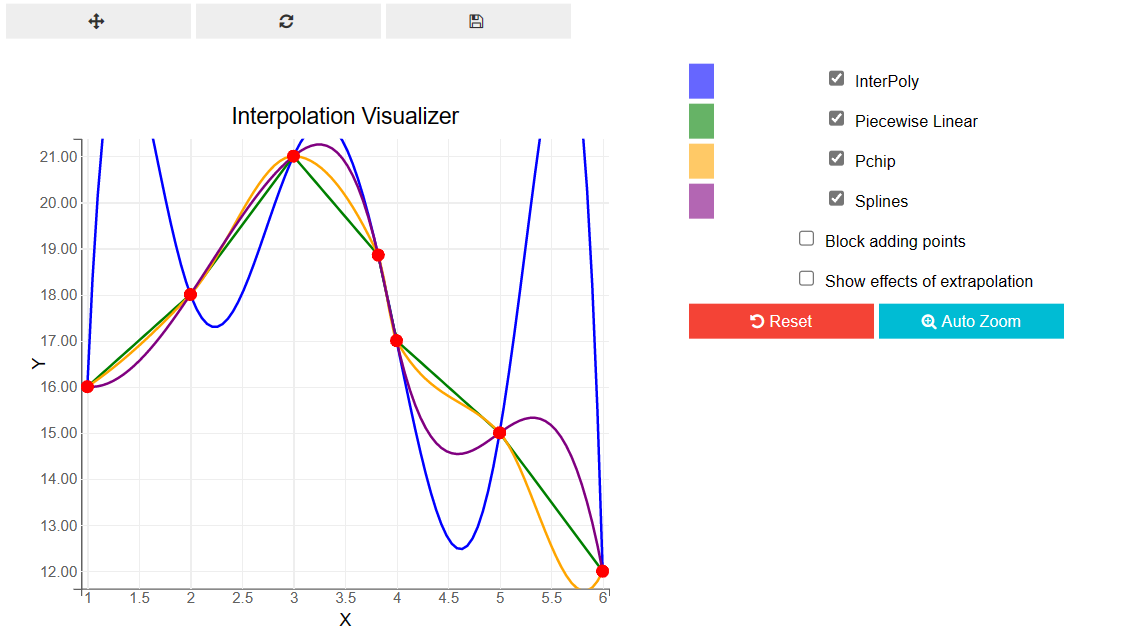
\includegraphics[scale=0.5]{Include/Images/Thesis/Documentation/Visualizers/Interpolation/Example 1/Example 1 - 03 - Added Point.png}

\item AutoZoom: \\
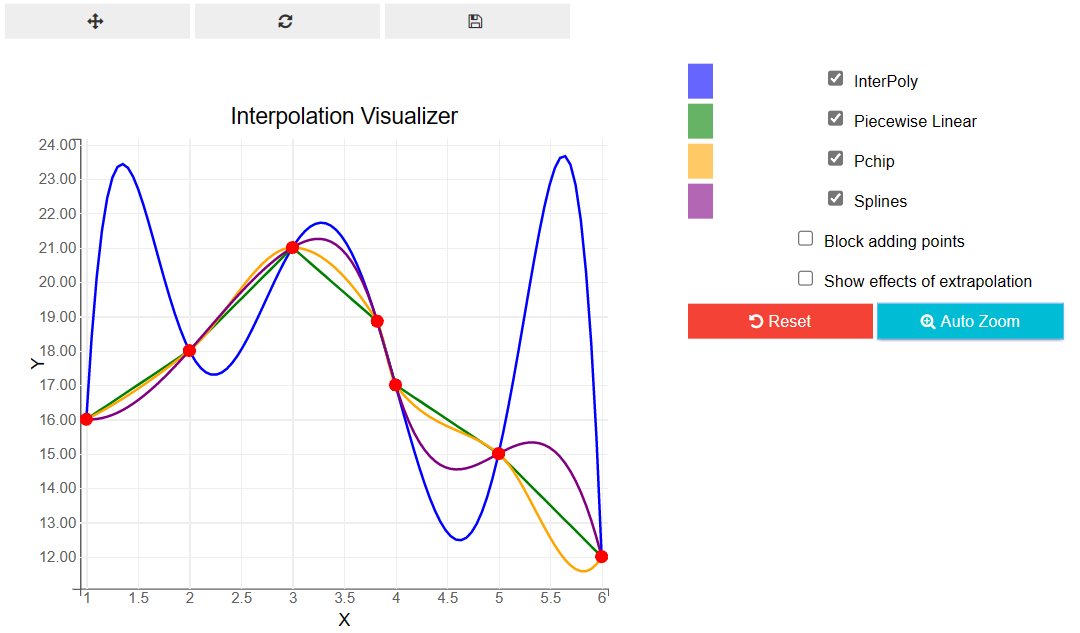
\includegraphics[scale=0.5]{Include/Images/Thesis/Documentation/Visualizers/Interpolation/Example 1/Example 1 - 04 -AutoZoom.png}
\end{enumerate}

\subsection{NonLinear Visualizer}

\subsection{Least Squares Visualizer}

\subsection{Random Numbers Visualizer}